\section{Simulación del NIOS II \label{sec:s1}}

\begin{center}
	\begin{minipage}{12cm}
		\begin{tcolorbox}[title=Actividad 1]
			Simular el sistema con procesador NIOS que incluya el puerto PIO, mostrar la salida de la consola y el visor de formas de onda del simulador ModelSim. La simulación debe imprimir un mensaje en la consola y escribir valores al puerto PIO de 8 bits.
		\end{tcolorbox}	
	\end{minipage}
\end{center}

En el entorno de \textit{Eclipse}, para la programación del procesador Nios II, se modificó el código en comparación con la Práctica 7, debido a que se necesitaba implementar un retardo menor para visualizar los valores a la salida. En la \autoref{fig:programmer} se observa la compilación del programa en C, con la respectiva modificación. Ahora bien, al momento de ejecutar el NIOS II en el entorno de ModelSim, se generó un archivo con terminación \textit{.do} que contiene la aplicación del \textit{reset} al sistema, la inicialización de las señales en la pestaña de formas de onda y el tiempo de simulación. En la \autoref{fig:wave} se visualiza la simulación de las señales, donde se tiene que al inicio el procesador requiere cerca de 60 $\mu$s para imprimir el texto en la consola (ver \autoref{fig:console}) y el tiempo restante es empleado para cargar los valores en el puerto paralelo de salida.

\begin{figure}[ht]
	\centering
	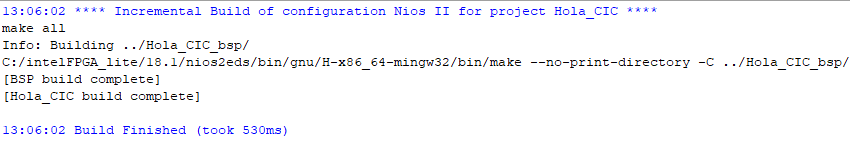
\includegraphics[scale=0.74]{NIOS_Console.png}
	\caption{Programación del procesador NIOS II con un retardo de 1 $\mu$s. \label{fig:programmer}}
\end{figure}

\begin{figure}[ht]
	\centering
	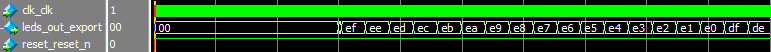
\includegraphics[scale=0.82]{ModelSim_Wave.png}
	\caption{Visualización de la salida del Procesador NIOS II en el visor de formas de onda de ModelSim (formato hexadecimal). \label{fig:wave}}
\end{figure}

\begin{figure}[ht]
	\centering
	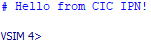
\includegraphics[scale=1.6]{ModelSim_Console.png}
	\caption{Impresión de una cadena de texto en la consola de ModelSim. \label{fig:console}}
\end{figure}